\section{On-chain voting and incentive}

Nebulas is dedicated to on-chain governance and is committed to using blockchain technology to provide a more open and collaborative environment.

\subsection{On-chain governance process}
\label{governance}

The general process of Nebulas' on-chain governance is as followed~\ref{fig:on-chain-governance}:

\begin{figure}
	\centering
	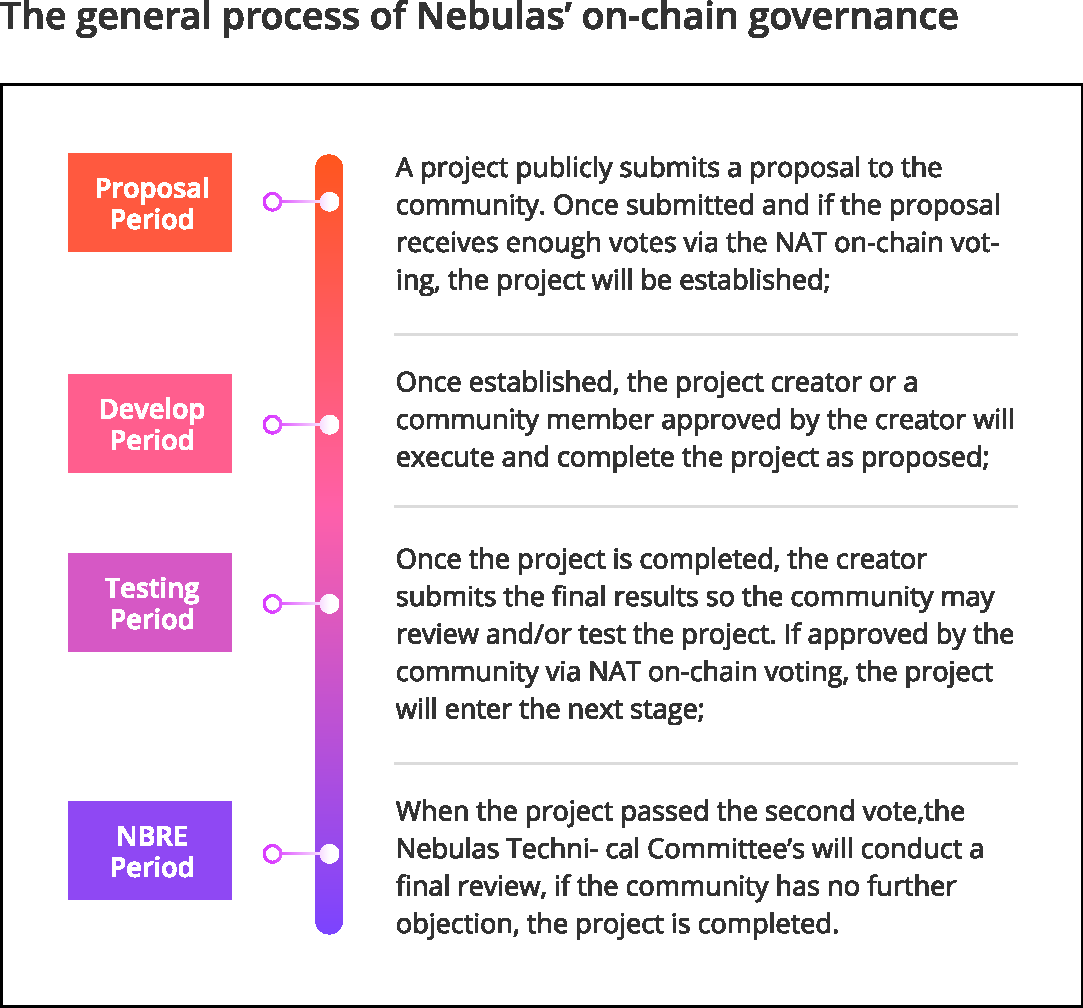
\includegraphics[width=1\textwidth]{../common/en/on-chain-governance.pdf}
	\caption{Nebulas on-chain governance process \label{fig:on-chain-governance}}
\end{figure}

\begin{enumerate}
	\item \textbf{Proposal Period}: A project publicly submits a proposal to the community. Once submitted and if the proposal receives enough votes via the NAT on-chain voting, the project will be established;
	\item \textbf{Develop Period}: Once established, the project creator or a community member approved by the creator will execute and complete the project as proposed;
	\item \textbf{Testing Period}: Once the project is completed, the creator submits the final results so the community may review and/or test the project. If approved by the community via NAT on-chain voting, the project will enter the next stage;
	\item \textbf{NBRE Period}: When the project passed the second vote, the Nebulas Technical Committee's will conduct a final review. If the community has no further objection, the project is completed.
\end{enumerate}

On-chain governance utilizes two components:

\begin{enumerate}
	\item Voting utilizes the NAT governance token and its underlying algorithms.
	\item The voting process is trust-less via blockchain technology.
\end{enumerate}

This Orange Paper will introduce the on-chain governance mainly.

\subsection{Basic principles of voting}

The Nebulas ecosystem integrates voting with its mainnet. Every vote cast by community members is transparent and visible for all to see. Within Nebulas, voting will utilize the following basic principles:

\begin{enumerate}
	\item The most basic unit of voting is a Nebulas mainnet address.
	\item The votes weight will refer to the address' Nebulas Rank score.
	\item Users positive contribution to the system should be rewarded with more voting rights. We believe that voting is a positive contribution to the Nebulas ecosystem and users should be motivated by receiving more voting rights.
\end{enumerate}

\subsection{Voting method}

Voting will be operated through a voting smart contract on the mainnet of the Nebulas blockchain. Each address can choose one of three options: For, Against or Abstain. Users can also choose not to vote.

\subsection{The only utilized voting medium: NAT}

\label{nat}

\subsubsection{Overview}

\begin{itemize}
	\item \textbf{Name}: Nebulas Autonomous Token
	\item \textbf{Ticker Symbol}: NAT
	\item \textbf{Form}: NRC20 token
\end{itemize}

The Nebulas Autonomous Token (NAT) is the asset derived from Nebulas Rank which will be embodied in the form of a NRC-20 token and will serve as the only voting medium within the Nebulas governance ecosystem.

\begin{center}
\fboxsep24pt
\colorbox{yellow!30}{
\begin{minipage}[c]{.8\textwidth}
	\paragraph{What is Nebulas Rank?}
	Nebulas Rank (NR) is the first on-chain, native, multidimensional value measurement mechanism for blockchain data.

  Within the Nebulas economy, the basic unit of governance is an \emph{address}
  (\ref{rights}). Nebulas Rank quantifies the contribution of each
  \emph{individual} to the economic accumulation via mathematical expression of
  the contribution to each address. Nebulas Rank is divided into \emph{Core
  Nebulas Rank} and \emph{Extended Nebulas Rank}. Core Nebulas Rank primarily reflects two factors:

	\begin{enumerate}
		\item The median value of the account within a certain period of time.
		\item The degree of asset utilization of the account over a period of time.
	\end{enumerate}

	At the macro level, the relationship between the number of currencies, value of money, rate of circulation, and productivity within the blockchain is described by the classical equation of the quantity of money in economics. The Nebulas Rank of the entire network can reflect the overall liquidity of the Nebulas ecosystem and its activity.


	\paragraph{NAT and NR}

  The release of NAT mainly refers to the \emph{Core Nebulas Rank} which is the asset performance. NAT issuance will review the calculated Nebulas Rank weekly with reference to the median and the degree of utilization of the assets within the week. For more information on the Nebulas Rank Score, please refer to the \textit{Yellow Paper - Nebulas Rank} published by the Nebulas Research Institute in June, 2018.


	\paragraph{How to check your Nebulas Rank?}

Nebulas Rank via Nebulas NOVA~\cite{nova} received its first upgrade on May 6, 2019. This upgrade utilized the Nebulas Blockchain Runtime Environment (NBRE) for autonomous and instant upgrades. The Nebulas Rank algorithm is open-sourced and can be checked online~\cite{CheckNR}.


\end{minipage}}
\end{center}

\subsubsection{Use cases of the Nebulas Autonomous Token (NAT)}


NAT is the only voting medium within Nebulas. Community members can vote on-chain via the NAT token to decide the direction of the Nebulas ecosystem. These decisions include but are not limited to: the election of Nebulas Council members, adjustments to the Nebulas Protocol Representation(NPR) via the Nebulas Blockchain Executable Environment (NBRE), establish, vote and review community proposals.

\subsubsection{Release}

The distribution method of NAT is similar to that of Bitcoin with the premise that there is an upper limit on the total supply and the distributed supply is decremented weekly.

The supply upper limit of NAT tokens is related to the Nebulas Rank score of
the entire Nebulas mainnet. The release amount is decremented weekly and the
attenuation coefficient is $\lambda$. The initial value of $\lambda$ is 0.997; this means that by week 180, the circulation is decremented to 58\% of the first week.

The initial circulation of NAT is based on the status of Nebulas NOVA mainnet after the completion of it's first voting upgrade on May 6th, 2019. Based on the current Nebulas Rank of the entire network and initial parameters, the upper limit of the total amount of NAT to ever exist will be 100 billion.

\subsubsection{Managing NAT}

Users can manage their NAT via NAS nano Pro~\cite{NASnano} and other wallets that support Nebulas NRC20~\cite{wallets} tokens. Users can view NAT transactions and circulation on blockchain explorers~\cite{explorer} that support the Nebulas mainnet.

\subsection{Obtaining NAT}

All users who control Nebulas mainnet addresses (with the exception of black listed address) have the opportunity to receive NAT. Address holders can obtain NAT via three ways: improve the Nebulas Rank score of the address, participate in Nebulas on-chain voting and by pleading NAS.


\paragraph{NAT blacklisted addresses}

During the NAT distribution process, any address that conflicts with any of
Nebulas \emph{address} basic rights (~\ref{rights}) will be classified as a blacklisted address.

Blacklist addresses can only obtain partial NAT based on their rights. For example, the address of a centralized exchange is classified as a blacklist address. According to the first basic right of Nebulas address owners, the address has the right to own and operate their assets on Nebulas; in return, the exchange address can obtain NAT under the same conditions according to the Nebulas Rank of the address. However, the collected property (NAT) of the exchange should be distributed to the corresponding exchange user. According to the second and third basic rights Nebulas address ownership, the exchanges collection address does not have the right to initiate a proposal or to participate in proposal vote before the exchange proves that the collection address fully represents the corresponding custody asset user proposal and voting willingness. Therefore, blacklisted addresses cannot obtain a NAT incentive by participating in the voting.


\subsubsection{Receive NAT by improving the Nebulas Rank score of an address}

NAT tokens will be distributed to Nebulas mainnet address which have a positive NR score on a weekly basis. The number of NAT tokens distributed will be based on the weekly Nebulas Rank of the address and the Nebulas Rank of the entire mainnet.

The number of distributed tokens will be decremented weekly. The attenuation coefficient is $\lambda$. Initially $\lambda$ = 0.997.

In the $i$th week, the ratio is:
\begin{align}
1\,\text{NR}=z(x_{ne},x_{e},\mu)\times\lambda^{i}\,\text{NAT}
\end{align}
Above Formula breakdown:

\begin{itemize}
	\item $\lambda$: attenuation coefficient.
	\item $\mu$: incentive parameters for voting behavior.
	\item $x_{ne}$: the sum of the NR score of non-exchange address on the entire mainnet.
	\item $x_{e}$: NR sum of the entire mainnet.
	\item $z(x_{ne},x_{e},\mu)$: function with $x_{ne}$, $x_{e}$ and $\mu$ as variables, Nebulas Rank and NAT redemption proportion.
\end{itemize}

\subsubsection{Pledging NAS to receive NAT}

Starting May 6, 2019, users of Nebulas mainnet can choose to obtain NAT by
\emph{pledging} Nebulas native coin NAS via a smart contract.

Users of the Pledge NAS smart contract will receive NAT beginning the second week after pledging begins (May 13, 2019). If users cancel their pledge, NAT distribution will cease.

The number of distributed tokens per week will be decremented. The attenuation coefficient is $\lambda$. Initially $\lambda$ = 0.997.

The ratio of pledge NAS to NAT during the $i$th week:
\begin{align}
x\,\text{NAS} \rightarrow \alpha \times z(x_{ne},x_{e},\mu)\times g(x) \times
  \lambda^{i}\,\text{NAT}
\end{align}
Above Formula breakdown:

\begin{itemize}
	\item $x$: the number of pledged NAS.
	\item $\alpha$: the pledge coefficient, $\alpha$=5 in the initial state.
	\item $z(x_{ne},x_{e},\mu)$: function with $x_{ne}$, $x_{e}$, and $\mu$ as variables, the exchange ratio of NR and NAT.
	\item $g(x)$: A function associated with $x$ that simulates the Nebulas Rank obtained by the NAS with a $x$ value on the Nebulas mainnet.
\end{itemize}


\paragraph{How to start pledging?}
To begin a pledge, users will need to send a transaction to the voting smart contract via their Nebulas wallet such as NAS nano Pro or other wallets that support the Nebulas mainnet. In return, the pledged NAS will be locked in the smart contract until the pledge is canceled by the user.

In order to guarantee the acquisition of NAT, the user must send their NAS to the Pledge smart contract address via a user controlled address which they hold the private key to. Users must not send NAS to the pledge smart contract directly from an exchange or address you do not fully control.


\paragraph{How to cancel pledging?}

If a user wants to cancel their pledge and unlock their NAS, NAS nano Pro or other supported wallets can interact with the smart contract to cancel the pledge. After canceling, the pledged NAS will be unlocked and will become available to the user.

\subsubsection{Receive NAT through Nebulas on-chain voting}

The NAT will be conducted at the beginning of every week on the Nebulas
mainnet. Once addresses obtain NAT, they can choose to vote on various
proposals and elections. Available voting options are \textit{For}, \textit{Against}, or
\textit{Abstain}; each choice is a valid option to receive incentives. If a user does not participate in any voting during the weekly cycle, they will not receive any additional incentives the following week.


\paragraph{Proportion of incentives}

The distribution and proportion of incentives should be fair and not used maliciously. To assist with these standards, the weekly NAT will look at the following:

\begin{enumerate}
	\item The number of NAT the address utilized for voting during the week.
	\item The amount of NAT tokens to be received this week based on the addresses' Nebulas Rank score from the previous week.
\end{enumerate}

If a person votes the amount of NAT that is smaller than or equal to the NAT that is distributed based on its NR, the voted NAT will be counted in the incentive algorithm, if a person votes the NAT that is larger than the NAT that is distributed based on its NR, this part will not be considered by the incentive algorithm. 

During the $i$th week, NAT incentive distribution on the maninet address, the following formula will be used:
\begin{align}
\mu \times \min \{N_{v}, N_{nr}\} \times \lambda^{i}
\end{align}
Above Formula breakdown:

\begin{itemize}
	\item $\mu$: the incentive parameters, $\mu$=10 under the initial parameters.
	\item $\lambda$: attenuation coefficient, initial value $\lambda$=0.997.
	\item $N_{v}$: the amount of NAT that is voted by the address during this week.
	\item $N_{nr}$: how much NAT the address will receive this week based on the previous week's Nebulas Rank score.
\end{itemize}
\noindent When $N_{v}$ (sent by the address in the week) is less than or equal
to $N_{nr}$, the number of incentive NAT obtained will be $\mu\times N_{v}$. When the $N_{v}$ of the address is greater than $N_{nr}$, the amount incentive obtained will be $\mu\times N_{nr}$.

\paragraph{For example}

An address obtains 10 NAT based on its NR score from the previous week and there is a total of 1,000 NAT held within the address.

This week, the address votes 5 NAT which is less than the 10 NAT received based on its NR score from the previous week, and in return, will receive $10\times5=50$ NAT voting incentive.

If the address votes 1,000 NAT which is more than received the past week (10 NAT) and in return will receive $10\times10=100$ NAT voting incentive.

\paragraph{}
Similar to the weekly NAT and the NAS pledge program, the distribution of the NAT voting incentive is also decremented weekly by the same coefficient. Under the initial parameters, $\lambda$, the attenuation coefficient is $\lambda$=0.997.

\subsection{Voting rules}

\subsubsection{Voting fee}

Each vote will be charged $\theta$\% NAT as a voting fee which is authorized by the Nebulas Council to be managed by the Nebulas Foundation as a special operating fund for the NAT project. The project team will not use the collected fee directly for voting. The initial voting fee value is $\theta$=3.

\subsubsection{Voting and NAT Destruction}

During each weekly release cycle, the NAT that users utilize on the Nebulas mainnet via the voting smart contract will be immediately destroyed. NAT tokens will however be distributed every week via the above listed methods to reduce the overall network destruction rate. The proportion of destruction will be decremented according to the cycle. The deceleration rate is consistent with the issuance rate of NAT. The NAT destroyed during each cycle will be calculated according to the NAT destruction rate function as shown in the appendix ref{burn}.

\subsubsection{Voting approval requirements}

For a proposal to be approved, the votes must meet two criterias: the degree of participation in voting and the proportion of votes in favor.

\begin{enumerate}
	\item

	\textbf{Voting engagement:}

	For proposals involving the use of public asset support, voting should not be less than the proportion of assets asked for by the proposal to account for assets in circulation across the network.

	If a proposal requires the use of $X$ NAS, the NAS in circulation on the
	  mainnet (any NAS that is not in the lock/pledge state and are available for
	  immediate transfer on the mainnet) is $Y$.

	Then the proposal must reach a voting participation rate not lower than
	  $X/Y$, which is converted into NAT; the ratio of the NAT participating in
	  the voting shall not be lower than $X/Y$.

	For proposals that do not involve the use of public asset support, voting participation is determined jointly by the community. Such proposals include but are not limited to: the adjustment of the mainnet parameters, the NPR to be performed by NBRE, etc...

	\item

	\textbf{The proportion of votes in favor:}

	In addition to meeting the minimum voting participation, the proportion of
	  votes required for a particular vote to be met must not be less than 51\%.
	  That is, assuming that a proposal receives a total of N votes, of which the
	  affirmative vote is Y, the negative vote is N and the abstention is A, the
	  proposal is considered to have been approved on only when $Y/(Y+N+A) \ge
	  51\%$.

\end{enumerate}

\subsection{Voting supervision and management}

\subsubsection{Voting process supervision}
\label{second-vote}

The Nebulas Technical Committee is appointed by the Nebulas Council to oversee the governance process and to ensure that the entire process is open and transparent. Public voting on Nebulas' public chain is organized and managed by the Nebulas Technology Committee.

Public voting accepts supervision from all members of the community. For proposals that violate any basic rights of any Nebulas address, the Nebulas Technical Committee may request a retrial of the proposal to the Nebulas Council. As the supervisor of the legitimacy of the governance process within the Nebulas ecosystem, the Nebulas Council has the right to file one and only one request for a \textbf{second vote}.

When the Board makes a request for a \emph{second vote}, the proposal is deemed to have entered a new voting cycleand the results of the first voting process are not executed. The NAT voted in the initial cycle will not be returned and will be burned according to the burn rate of the cycle.

The voting participation of the second vote must be greater than the
participation of the first vote. That is to say, if the participation degree of
the first vote is $X/Y$, the participation degree of the second vote should be
greater than $X/Y$, and the proportion of the votes in favor must not be less than 51\%.

\subsubsection{NAT parameter adjustment}

The NAT distribution process involves the following factors:

\begin{enumerate}
	\item $\alpha$: pledge coefficient, initial value $\alpha$=5
	\item $\mu$: voting reward factor, initial value $\mu$=10
	\item $\lambda$: attenuation coefficient, initial value $\lambda$=0.997
	\item $\theta$: voting fee, initial value $\theta$=3
\end{enumerate}

Adjustment of the coefficient must go through the governance voting process; the Nebulas Foundation or NAT project team has no right to adjust the coefficients without authorization.
